\chapter{Differential Analysis}

\section{Mass Conservation}
{\footnotesize\textit{Munson 6.2}}
Recall the law for mass conservation that was transferred to a control volume approach in the last chapter:
\begin{equation*}
	\begin{split}
		\frac{dM_{sys}}{Dt}&=0\\
		\text{\footnotesize Reynolds Transport Theorem:} \quad \frac{\partial}{\partial t}\int_{cv} \rho \,dV + \underbrace{\int_{cs} \rho \vec v \cdot \hat n\,dA}_{\stackrel{\text{Gauss}}{=} \int_{cv} \nabla \cdot (\rho \vec v )\,dV} &= 0\hfill\\
		\int_{cv} \left[\frac{\partial}{\partial} \rho + \nabla \cdot (\rho \vec v)\right]\,dV &= 0 \stackrel{(*)}\Longleftrightarrow \frac{\partial}{\partial} \rho + \nabla \cdot (\rho \vec v)=0
	\end{split}
\end{equation*}
Where at $(*)$ we figure that an integral over an arbitrary volume can only be zero if the integrand itself is zero.
The resulting equation is what we call the \textbf{continuity equation}:
\begin{equation*}
	\boxed{\frac{\partial \rho}{\partial t} + \nabla \cdot \left(\rho \vec v \right) = 0}\qquad \text{Eularian Form}
\end{equation*}
The Lagrangian form is as follows:
\begin{equation*}
	\boxed{\frac{D\rho}{Dt} + \rho \nabla \cdot \vec v = 0} \qquad \text{Lagrangian Form}
\end{equation*}

For an incompressible case, where $\rho = const$, then 
\begin{equation*}
	\boxed{\nabla \cdot \vec v = 0}  \qquad \text{Incompressible}
\end{equation*}




\section{Navier-Stokes Equations (Momentum Conservation / Newtons \nth2 law)}
{\footnotesize\textit{Munson 6.3}}  Recall newtons \nth2 law for a Lagrangian system, which we rewrote to an eularian fashion:
\begin{equation*}
	\frac{D}{Dt} (M\vec v)_{sys} = \sum \vec F_{ext}\implies \frac{\partial}{\partial t} \int_{cv}\rho\vec v \,dV + \int_{cs}\rho \vec v (\vec v \cdot \hat n) = \sum \vec F_{ext}
\end{equation*}
As before, we would like to rewrite everything under one volume integral. 

The second term can be rewritten using Gauss:
\begin{equation*}
	\int_{cs} \rho \vec v(\vec v \cdot \hat n) \,dA \stackrel{\text{Gauss}}{=} \int_{cv} \nabla\cdot (\vec v \rho \vec v)\,dV
\end{equation*}
Since $\rho$ is constant, we can denote the $i$th component of the integrand as 
\begin{equation*}
	\nabla\cdot (\vec v \rho \vec v)\stackrel{\nabla \cdot \vec v = 0}= \rho v_j \partial_j v_i = \rho \vec v \cdot \nabla \vec v
\end{equation*}

For a control volume, we want to consider the following forces (right hand term):
\begin{itemize}
	\setlength{\itemsep}{-5pt}
	\item \textbf{body forces}
	\begin{equation*}
		\int_{cv} \rho \vec g \,dV
	\end{equation*}
	\item \textbf{surface forces} (including non-viscous forces)
	
	The non-viscous force is pressure acting on the differential element. non-viscous forces are represented in the rank two stress tensor $\overline{\overline{\tau}}$:
	\begin{equation*}
		\overline{\overline{\tau}} = \begin{pmatrix}
			\tau_{xx}&\tau_{xy}&\tau_{xz}\\
			\tau_{yx}&\tau_{yy}&\tau_{yz}\\
			\tau_{zx}&\tau_{zy}&\tau_{zz}\\
		\end{pmatrix}
	\end{equation*}
	The stress tensor has the following properties:
	\begin{itemize}
		\item $\hat n \cdot \overline{\overline{\tau}}$ or $(\hat n \cdot \overline{\overline{\tau}})_j = n_i\tau_{ij}$ is the stress on the surface with normal $\hat n$.
		\item $\tau_{ij} = \tau_{ji}\implies \hat n \cdot \overline{\overline{\tau}}  = \overline{\overline{\tau}} \hat n$ (symmetric)
	\end{itemize}
	We define the cauchy stress tensor $\overline{\overline \sigma}\cdot \hat n$ with $\overline{\overline \sigma} = -p\overline{\overline{I_d}} + \overline{\overline{\tau}}$ All surface forces combined can therefore be expressed as
	\begin{equation*}
		\int_{cs} \overline{\overline \sigma }\cdot \hat n  \,dA = \int_{cv} \nabla \cdot \overline{\overline {\sigma}}\,dV
	\end{equation*}
\end{itemize}

The complete volume integral with all terms is
\begin{equation*}
	\int_{cv}\rho\frac{\partial \vec v}{\partial t} + \rho \vec v \cdot \nabla \vec v - \rho \vec g - \nabla \cdot (-p\overline{\overline{I_d}}+ \overline{\overline{\tau}}) \,dV = 0
\end{equation*}
Which is valid for all control volumes, and therefore the integrand must also be zero. This is the \textbf{Cauchy's Equation}:
\begin{equation}
\boxed{\rho \left(\frac{\partial \vec v}{\partial t} + \vec v \cdot \nabla \vec v \right) =-\nabla p + \rho \vec g + \nabla \cdot \overline{\overline{\tau}}}
\end{equation}



Recall the result for a Newtonian fluid:
\begin{equation*}
	\tau = \mu \frac{dv_x}{dy} = \tau_{yx}=\tau_{xy}
\end{equation*}
We now know that this $\tau$ is a component of the stress-strain tensor $\overline{\overline{\tau}}$. We were looking at the surface $y$ in the velocity in $x$. We can therefore express the stress-strain rate relationship (which is linear) for a more complicated geometry, as
\begin{equation*}
	\tau_{ij} = \mu \left(\frac{\partial v_i}{\partial x_j} + \frac{\partial v_j}{\partial x_i}\right)
\end{equation*}

Through this new relation, we can substitute into Cauchy's Equation:
\begin{equation*}
	(\nabla \cdot \overline{\overline{\tau}})_j = \partial_i\tau_{ij} = \mu \left(\cancel{\partial_i\partial_j v_i} + \partial_i \partial_i v_j\right) = \mu \nabla^2v_j
\end{equation*}
We could cancel the first term due to mass conservation for incompressible fluids ($\nabla \cdot \vec v = 0$).
this yields

\resizebox{\textwidth}{!}{\shadowbox{$\displaystyle
		{\boxed{\rho \left(\frac{\partial \vec v}{\partial t} + \vec v \cdot \nabla \vec v \right) =-\nabla p + \rho \vec g + \mu \nabla^2\vec v}} \qquad \substack{\text{Navier-Stokes Equation}\\\text{(Incompressible flow)}}
		$}}
	
For an incompressible Newtonian fluid with $\rho = const, \mu = const$, 
we can summarise:
\begin{equation*}
	\begin{cases}
		\rho \left(\frac{\partial \vec v}{\partial t} + \vec v \cdot \nabla \vec v \right) =-\nabla p + \rho \vec g + \mu \nabla^2\vec v\\
		\nabla \cdot \vec v = 0
	\end{cases}
\end{equation*}
Together with boundary and initial conditions, this describes all fluid mechanics problems of Newtonian fluids.
We cannot solve it however.

In order to make progress, we can solve it for a set of special cases.
  
\section{Inviscid Flow}
Looking at the Navier-Stokes Equation, we want to find out in which cases it is okay to neglect the inertial term and the viscous term:
\begin{equation*}
	\rho \frac{\partial \vec v}{\partial t} + \underbrace{\cancel{\rho \vec v \cdot \nabla \vec v}}_{\substack{\text{inertial /}\\\text{advection term}}}  = -\nabla p + \rho g + \underbrace{\cancel{\mu \nabla^2 \vec v}}_{\substack{\text{viscous}\\\text{term}}}
\end{equation*}
We want to understand the "scaling" in order to estimate the terms:
\begin{itemize}
	\setlength{\itemsep}{-5pt}
	\item \textbf{viscous term:} $|\mu\nabla^2 \vec v| \approx \mu \cdot \frac{V}{L^2}$
	\item \textbf{inertial term:} $|\rho \vec v \cdot \nabla \vec v|\approx \rho \cdot \frac{V^2}{L}$
\end{itemize}
where $V$ is the characteristic velocity and $L$ is the length.
We define the Reynolds number:
\begin{equation*}
	Re := \frac{\text{"inertial term"}}{\text{viscosity}} = \frac{\rho V^2/L}{\mu V/L^2} = \frac{VL}{\mu/\rho} = \frac{VL}{\nu}
\end{equation*}
where $\nu$ was the kinematic viscosity.
We can conclude that:
\begin{itemize}
	\setlength{\itemsep}{-5pt}
	\item With a \textbf{large Reynolds number} ($Re >> 1$), we can justify to neglect the \textbf{viscous term}\footnote{The term we dropped, we changed the order of the equation from 2 to one: we therefore cannot apply all boundary conditions.}:
	\begin{equation*}
		\boxed{\rho \frac{\partial \vec v}{\partial t} + \rho \vec v \cdot \nabla \vec v =-\nabla p + \rho \vec g }\qquad \substack{\text{Euler Equation}\\\text{"inviscid flow"}}
	\end{equation*}
	\item With a \textbf{small Reynolds number} ($Re << 1$), we can justify to neglect the \textbf{inertial term}
	\begin{equation*}
		\boxed{\rho \frac{\partial \vec v}{\partial t} =-\nabla p + \rho \vec g + \mu \nabla^2\vec v}\qquad \substack{\text{Stoke's Equation}\\\text{"creeping flow"}}
	\end{equation*}
\end{itemize}

\section{Vorticity and Circulation}
\paragraph{Deformation of a Fluid Element:} Let's consider a fluid element as a box with a certain size $\delta x, \delta y, \delta z$. It is advected in the fluid flow. If the velocity would be uniform, then the fluid element would just be transported without deforming. If not (i.e. the corners of the box don't have the same velocity), it will deform. \textit{The deformation is controlled by the velocity gradients with space}.

\begin{itemize}
	\setlength{\itemsep}{-5pt}
	\item \textbf{linear deformation}: (diagonal components of the gradient velocity tensor)
	\begin{figure}[H]
		\centering
		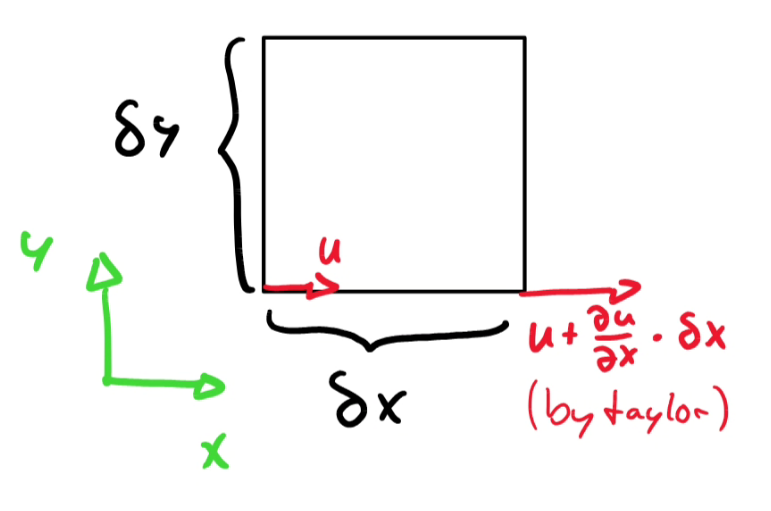
\includegraphics[width=0.4\linewidth]{Sketches/LinearDeformation}
		\caption{}
		\label{fig:lineardeformation}
	\end{figure}
	\begin{equation*}
		\frac{d(\delta x)}{d t} = \frac{\partial u}{\partial x} \implies \frac{1}{\delta x} \frac{d (\delta x)}{d t} = \frac{\partial u}{\partial x}
	\end{equation*}
	Likewise, $\partial_y v, \partial_z w$ are the linear deformations in $y$ and $z$, respectively. The volume change $\delta V = \delta x\cdot \delta y \cdot \delta z $ can be expressed as:
	\begin{equation*}
	\begin{split}
		   \frac{1}{\delta V}\frac{d(\delta V)}{dt}  
		&= \frac{1}{\delta x}\frac{d(\delta x)}{dt} + \frac{1}{\delta y}\frac{d(\delta y)}{dt}+\frac{1}{\delta z}\frac{d(\delta z)}{dt} \\
		&= \frac{\partial u}{\partial x} + \frac{\partial v}{\partial y } + \frac{\partial w}{\partial z}\\
		&= \nabla \cdot \vec v = 0\text{, if $\rho=const$}
	\end{split}
	\end{equation*}
	\item \textbf{angular deformations} (off-diagonal components of the gradient velocity tensor)
	\begin{figure}[H]
		\centering
		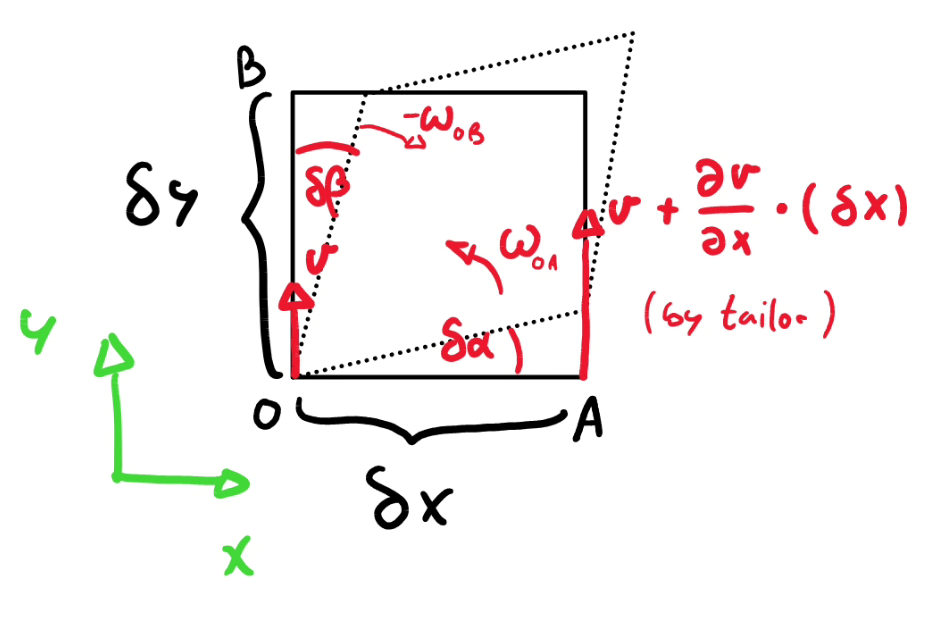
\includegraphics[width=0.4\linewidth]{Sketches/angular_deformations}
		\caption{}
		\label{fig:angulardeformations}
	\end{figure}
	\begin{equation*}
		\begin{split}
			\omega_{OA} &= \lim_{\Delta t \to 0}  \frac{\delta \alpha}{\Delta t} \stackrel{(*)}= \lim_{\Delta t \to 0} \frac{1}{\Delta t} \left(\frac{\frac{\partial v}{\partial x}\delta x \Delta t}{\delta x}\right) = \frac{\partial v}{\partial x}\\
			\omega_{OB} &= -\frac{\partial u}{\partial y}
		\end{split}
	\end{equation*}
	At $(*)$ we used a small angle approximation $\tan\delta \alpha \approx \delta \alpha$. The average rotation is the rotation of the bisecting line $\overline {OC}$. We can write it's angular velocity as
	\begin{equation*}
		\omega_z = \frac 12 \left(\omega_{OA}+\omega_{OB}\right) = \frac 12 \left(\frac{\partial v}{\partial x} - \frac{\partial u}{\partial y}\right)
	\end{equation*}
	Applying the same around $x$ and $y$ axis yields
	\begin{equation*}
		\vec \omega = \frac 12 \nabla \times \vec v = \frac 12 \zeta
	\end{equation*}
	in terms of the is the \textbf{vorticity} $\zeta$:\footnote{Heads up: Vorticity is not necessarily a circular transportation, but rather if (and how much) the fluid elements rotate about \textbf{their own axis}.}
	\begin{equation*}
		\boxed{\zeta = \nabla \times \vec v}
	\end{equation*}
	\textbf{Circularity} is a measure of velocity on some curve $c$ around an area $A$ on the surface of a volume.
	\begin{equation*}
		\Gamma = \oint_{c} \vec v \cdot \vec{ds} = \oint_{A} (\nabla \times \vec v )\cdot \vec{dA}
	\end{equation*}
	Where we see the vorticity again.
	It can be shown that inviscid flow means no change in rotation ($d\Gamma/dt=0$) and we say that "$\Gamma$ is conserved".
	
	It is therefore reasonable to consider inviscid flows ($\mu \to 0$) and irrotational flows ($\nabla \times \vec v = \vec 0$).
\end{itemize}


\section{Potential flow / Irrotational flow}
We assume that we are looking at \textit{incompressible, inviscid, and irrotational} flow.
We know that
\begin{equation*}
	\nabla \times \vec v = \vec 0\implies \exists \phi : \vec v = \nabla \phi
\end{equation*}
with the velocity potential $\phi$.

The continuity, and momentum equations turn into:
\begin{equation*}
	\begin{split}
		\text{Continuity Equation}\qquad\qquad\qquad\qquad\quad \nabla \cdot \vec v &= 0 \qquad (\rho = const) \\
		&\implies \boxed{\nabla^2 \phi = 0}\\\\
		\text{Momentum balance}\qquad\,\,\qquad \rho \left(\frac{\partial \vec v}{\partial t}+ \vec v \cdot \nabla \vec v \right) &= \rho \vec g - \nabla p \qquad \\
		\implies  \rho \frac{\partial \phi}{\partial t} + \frac{\rho}{2}v^2 + p + \rho g z &= const \qquad \Big | \text{steady:} \partial_t \phi = 0\\		
		\frac{\rho}{2}v^2 + p + \rho g z &= const
	\end{split}
\end{equation*}
Note that the result from the momentum balance is the same as the Bernoulli equation, but not restricted to any field lines.

To solve such a problem we follow the following steps:
\begin{enumerate}
	\setlength{\itemsep}{-5pt}
	\item \textbf{Solve Laplace} $\nabla^2\phi = 0$ with appropriate boundary conditions
	\item \textbf{Compute Velocity} $\vec v = \nabla \phi\implies \phi, \vec v$ known
	\item \textbf{Solve for the Pressure} Solve the momentum balance $\frac{\rho}{2}v^2 + p + \rho g z = const$ for pressure.
	\item \textbf{Integrate Pressure over Surface} to get the force on the object
\end{enumerate}


\section{2D Flows -- The Stream Function}
We start from the conservation of mass in an incompressible situation:
\begin{equation*}
	\begin{split}
		\nabla \cdot \vec v &= 0, \vec v = u\hat i + v\hat j + \cancel{w\hat k}\\
		\nabla \cdot \vec v &= 0 \Leftrightarrow \frac{\partial u}{\partial x} = - \frac{\partial v }{\partial y}\\
		\exists \Psi(x,y) :  \frac{\partial \Psi}{\partial y} &= u, -\frac{\partial \Psi}{\partial x} = v\implies \nabla \vec v = \frac{\partial}{\partial x}\frac{\partial \Psi}{\partial y} - \frac{\partial}{\partial y} \frac{\partial \Psi}{\partial x} = 0
	\end{split}
\end{equation*}
The 2D velocity fields can be derived from a so-called \textit{stream-function} $\Psi$ that by construction satisfies mass conservation ($\nabla \cdot \vec v = 0$).



\section{2D Potential Flow}

\subsection{Basic plane potential flows}
\subsection{Superpositions}
\subsection{Lift and drag on an Airfoil}